\documentclass[10pt, a4paper, italian]{article}
\usepackage[T1]{fontenc}
\usepackage[utf8]{inputenc}
\usepackage{amsmath, amssymb, amsthm, thmtools, amsfonts, mathtools}
\usepackage{nicefrac}
\usepackage{calc}
\usepackage[pdftex, hyperindex, plainpages=false]{hyperref}
\usepackage[nameinlink]{cleveref} %load before classicthesis (clash)
%\usepackage[nochapters,pdfspacing]{classicthesis}
\usepackage{siunitx}
\usepackage[siunitx]{circuitikz}

\usepackage[a4paper]{geometry}
\usepackage{float}
\usepackage{mdframed}
\usepackage{titling}
\usepackage{booktabs}
\usepackage{graphicx}
\usepackage{caption, subcaption}
\usepackage{xcolor}
\usepackage[italian]{babel}
\usepackage{pgfplots}
\usepackage{listings}
%\usepackage{lmodern}
\usepackage{url}
\usepackage{enumitem}
\usepackage{tikz} %loads after classicthesis (xcolor incompat)

% lets graphicx know path where figures to be included are found
\graphicspath{{../figs/}}
\makeatletter
\def\input@path{{../figs/}}
%or: \def\input@path{{/path/to/folder/}{/path/to/other/folder/}}
\makeatother

% tikz pgf plots setup
\usepgfplotslibrary{external}
\pgfplotsset{compat=1.15}
%\tikzexternalize

% spaces and significant digits/figures for measurements
\sisetup{free-standing-units, space-before-unit, number-unit-product = \;,
scientific-notation = false, round-mode = figures, round-precision = 1,}

% turns all (hyperlinked) references black [default is blue]
\hypersetup{
	linktoc=all,
	colorlinks=true,
	linkcolor=black
}

% code listings config
%\lstset{
%language=Python,
%basicstyle=\ttfamily,
%columns=fullflexible,
%keepspaces=true,
%}

% mdframed (for boxed text) configuration
\mdfsetup{linewidth=0.6pt}

% Default fixed font does not support bold face
\DeclareFixedFont{\ttb}{T1}{txtt}{bx}{n}{12} % for bold
\DeclareFixedFont{\ttm}{T1}{txtt}{m}{n}{12}  % for normal

% Custom colors
\usepackage{color}
\definecolor{deepblue}{rgb}{0,0,0.5}
\definecolor{deepred}{rgb}{0.6,0,0}
\definecolor{deepgreen}{rgb}{0,0.5,0}

% Commands 
\newcommand{\executeiffilenewer}[3]{%
	\ifnum\pdfstrcmp{\pdffilemoddate{#1}}%
		{\pdffilemoddate{#2}}>0%
	{\immediate\write18{#3}}\fi%
}
% input .svg --> .pdf_tex graphs
%\newcommand{\includesvg}[1]{%
%	\executeiffilenewer{#1.svg}{#1.pdf}%
%	{inkscape -z -D --file=#1.svg %
%	--export-pdf=#1.pdf --export-latex}%
%	\input{#1.pdf_tex}%
%}
% Thanks UniPi's Department of Physics E. Fermi
\newcommand{\thanksdf}{(\thanks{Dipartimento di Fisica E.~Fermi,%
Universit\`a di Pisa - Pisa, Italy.}\;)}

% hyperlink to email address
\newcommand{\mail}[1]{\href{mailto:#1}{\textsf{#1}}}

% \vec for bold vectors, instead of overarrows (now "\arrvec")
\let\arrvec=\vec
\renewcommand{\vec}[1]{\boldsymbol #1}
% replaces straight phi with slanted phi
\renewcommand{\phi}{\varphi}
% replaces straight eps with curved epsilon
\newcommand{\eps}{\varepsilon}
% abbreviation for (sub_/super^)scripts of \lim, \sum,... in inline math
\newcommand{\ds}{\displaystyle}

% blackboard/number set letters
\newcommand{\CC}{\mathbb C}
\newcommand{\HH}{\mathbb H}
\newcommand{\KK}{\mathbb K}
\newcommand{\NN}{\mathbb N}
\newcommand{\PP}{\mathbb P}
\newcommand{\QQ}{\mathbb Q}
\newcommand{\RR}{\mathbb R}
\newcommand{\ZZ}{\mathbb Z}

\newcommand{\Abs}[1]{{\left\Vert #1\right\Vert}}
\newcommand{\enclose}[1]{{\left( #1 \right)}}
\newcommand{\Enclose}[1]{{\left[ #1 \right]}}
\newcommand{\floor}[1]{\left\lfloor #1 \right\rfloor}
\newcommand{\ceil}[1]{\left\lceil #1 \right\rceil}
\newcommand{\To}{\rightrightarrows}

% Math operators
\DeclareMathOperator{\divergence}{div}
\renewcommand{\div}{\divergence}
\DeclareMathOperator{\Imaginarypart}{Im}
\renewcommand{\Im}{\Imaginarypart}
\DeclareMathOperator{\Realpart}{Re}
\renewcommand{\Re}{\Realpart}
%\DeclareMathOperator{\arg}{arg}
\DeclareMathOperator{\tg}{tg}
\DeclareMathOperator{\arctg}{arctg}
\DeclareMathOperator{\settsinh}{settsinh}
\DeclareMathOperator{\settcosh}{settcosh}
\DeclareMathOperator{\tr}{tr}
\DeclareMathOperator{\im}{im}
\DeclareMathOperator{\sgn}{sgn}
\DeclareMathOperator{\diag}{diag}

\DeclarePairedDelimiter{\norm}{\lVert}{\rVert}
\DeclarePairedDelimiter{\scalar}{\langle}{\rangle}

% Logarithm with arbitrary base.
% -> log_10
\newcommand{\llog}[1][10]{\log_{#1}}

% Absolute value.
% -> |x|
\newcommand{\abs}[1]{\left| #1 \right|}

% Powers.
% -> x^a
\newcommand{\power}[2][2]{\left( #2 \right)^{#1}}

% Square.
% -> x^2
\newcommand{\sq}[1]{\power[2]{#1}}

% Expansion of the binomial coefficient.
% -> n1!/(n2!(n1 - n2)!)
\newcommand{\binomexpr}[2]{\frac{#1!}{#2!(#1 - #2)!}}

% Expression evaluation at a given point with square brackets.
% -> [x]_{a}
\newcommand{\at}[2]{\left[ #1\right]_{\makebox[-1pt][l]{${\scriptstyle#2}$}}}

% Expression evaluation in an interval.
% -> [x] _{a}^{b}
\newcommand{\eval}[3]{\left.#1%
  \right|_{\makebox[-1pt][l]{${\scriptstyle#2}$}}^{\makebox[-1pt][l]{${\scriptstyle#3}$}}}

% Upright d in math mode (for differentials).
% -> d
\newcommand{\ud}{\mathrm{d}}

% Differential.
% -> dx
\newcommand{\diff}[1][x]{\,\ud{#1}}

% Base command for defining derivatives.
% -> df/dx or d^kf/dx^k
\newcommand{\basederivative}[4][]{%
  \displaystyle%
  \ifx\\#1\\\frac{#4#2}{#4#3}%
  \else%
  \frac{#4^#1#2}{#4#3^#1}%
  \fi%
}

% Total derivative.
% -> df/dx(x) or d^kf/dx^k(x)
\newcommand{\td}[4][]{%
  \basederivative[#1]{#2}{#3}{\ud}%
  \ifx\\#4\\%
  \else%
  \mkern-4mu\left(#4\right)%
  \fi%
}

% Partial derivative.
% -> df/dx(x) or d^kf/dx^k(x)
\newcommand{\pd}[4][]{%
  \basederivative[#1]{#2}{#3}{\partial}%
  \ifx\\#4\\%
  \else%
  \mkern-4mu\left(#4\right)%
  \fi%
}

\newcommand{\intinf}{\int_{-\infty}^{\infty}\!\!\!}

\newcommand{\cinterval}[2]{\left[\, #1,~#2 \,\right]}

\newcommand{\linterval}[2]{\left[\, #1,~#2 \,\right)}

\newcommand{\rinterval}[2]{\left(\, #1,~#2 \,\right]}

\newcommand{\ointerval}[2]{\left(\, #1,~#2 \,\right)}

\newcommand{\prob}[1]{\displaystyle P\left(#1\right)}

\newcommand{\pvalue}{\emph{$p$-value}}

\newcommand{\cond}{\,|\,}

\newcommand{\expect}[1]{\displaystyle E\left[#1\right]}

\newcommand{\mom}[2][]{\displaystyle {\cal M}_{#2}\ifx\\#1\\\else(#1)\fi}

\newcommand{\momalg}[1]{\displaystyle \lambda_{#1}}

\newcommand{\momcen}[1]{\displaystyle \mu_{#1}}

\newcommand{\skewness}{\displaystyle \gamma_1}

\newcommand{\kurtosis}{\displaystyle \gamma_2}

\newcommand{\charf}[1][x]{\phi_{#1}}

\newcommand{\momgenf}[1][x]{M_{#1}}

\newcommand{\fwhm}{{\scriptstyle \textsc{FWHM}}}

\newcommand{\hwhm}{{\scriptstyle \textsc{HWHM}}}

\newcommand{\median}{\mu_{\nicefrac{1}{2}}}

\newcommand{\var}[1]{\ensuremath{\text{Var}\left(#1\right)}}

\newcommand{\cov}[2]{\ensuremath{\text{Cov}\left(#1, #2\right)}}

\newcommand{\corr}[2]{\ensuremath{\text{Corr}\left(#1, #2\right)}}

\newcommand{\like}{\mathcal L}

\newcommand{\likelihood}[2][]{\like\ifx\\#2\\\else(#2\ifx\\#1\\\else;#1\fi)\fi}

\newcommand{\chisq}{\ensuremath{\chi^2}}

\newcommand{\chisquare}[2][]{\chisq\ifx\\#2\\\else(#2\ifx\\#1\\\else;#1\fi)\fi}

\newcommand{\loglikelihood}[2][]{\log\likelihood[#1]{#2}}

\newcommand{\pdf}[3][]{#2(#3\ifx\\#1\\\else;#1\fi)}

\newcommand{\binomialpdf}[2][]{\pdf[#1]{\mathcal B}{#2}}

\newcommand{\multinomialpdf}[2][]{\pdf[#1]{\mathcal M}{#2}}

\newcommand{\poissonpdf}[2][]{\pdf[#1]{\mathcal P}{#2}}

\newcommand{\uniformpdf}[2][]{\pdf[#1]{u}{#2}}

\newcommand{\exponentialpdf}[2][]{\pdf[#1]{\varepsilon}{#2}}

\newcommand{\gausspdf}[2][]{\pdf[#1]{N}{#2}}

\newcommand{\chisquarepdf}[2][]{\pdf[#1]{\wp}{#2}}

\newcommand{\cauchypdf}[2][]{\pdf[#1]{c}{#2}}

\newcommand{\erf}[1]{\ensuremath{\text{erf}\left(#1\right)}}

\newcommand{\dccases}[4][]{#2 \ifx\\#2\\\else=\fi %
  \begin{cases}
    \displaystyle #3 & \text{per variabili discrete}\\
    \displaystyle #4 & \text{per variabili continue}#1
  \end{cases}
}
% sub/super-scriptable for all symbol as math operator 
\newcommand\Scaleforall[1]{\vcenter{\hbox{\scalefont{#1}$\forall$}}}

\DeclareMathOperator*\forevery{%
  \vphantom\sum
  \mathchoice{\Scaleforall{2}}{\Scaleforall{1.4}}{\Scaleforall{1}}{\Scaleforall{0.75}}}
\geometry{left=2cm, right=2cm, top=2cm, bottom=2cm}

% makes all hyperlinks the same color as text
\hypersetup{
	linktoc=all,
	colorlinks=false,
	linkcolor=black
	}
% lets graphicx know path where figures to be included are found
\graphicspath{{../figs/}}

\author{Gruppo 1.AC \\ Matteo Rossi, Bernardo Tomelleri}
\title{Es12: Misura del rapporto $h/e$ per effetto fotoelettrico}
\begin{document}
\date{\today}
\maketitle

%=======================
\section{Scopo dell'esperienza}
Scopo dell'esperienza è verificare l'effetto fotoelettrico e la dipendenza
lineare tra energia e frequenza dei fotoni, dunque da questa ricavare una stima
del rapporto tra la costante di Planck e la carica dell'elettrone $h/e$
utilizzando il metodo del potenziale frenante (implementato per la prima volta
da R.A. Millikan, 1914-16).

\section{Metodo di misura del potenziale frenante}
L'effetto fotoelettrico prevede che un elettrone può essere estratto da un
metallo assorbendo un fotone con energia superiore al lavoro di estrazione
$W_{0}$ e venire emesso con energia cinetica pari a
\begin{equation}\label{eq: cons}
E = h \nu - W_0
\end{equation}
dove $\nu$ è la frequenza della radiazione elettromagnetica incidente sul
metallo e $h \nu$ l'energia trasportata da ogni fotone di cui è costituita.

Nel nostro apparato sperimentale i \emph{fotoelettroni}, i.e. gli elettroni
estratti per effetto fotoelettrico dal catodo di una cella fotoelettrica
Leybold 5587 determinano una \emph{fotocorrente} verso l'anodo, che
colleghiamo all'ingresso di un picoamperometro (mod. Keithley 595: Quasistatic
C-V Meter) per riuscire a misurarne l'intensità $I_{ph}$.

Questi elettroni vengono `frenati' da un campo elettrico di verso concorde al
loro moto, generato da una tensione regolabile $V\ped{bias}$ applicata tra
anodo e catodo, al fine di trovare la differenza di potenziale critica $V_0$
per cui l'intensità di corrente $I_{ph}(V\ped{bias})$ si annulla.
La barriera di potenziale $eV_0$ corrispondente alla tensione che arresta il
flusso di fotoelettroni ci fornisce quindi una stima della massima
energia cinetica da essi raggiunta, che possiamo mettere in relazione alla
frequenza della radiazione incidente (per conservazione dell'energia
\cref{eq: cons})
\begin{equation}\label{eq: V0}
V_0 = \frac{h}{e} \nu - \frac{W_0}{e}
\end{equation}

Questa è proprio la relazione lineare tra energia e frequenza che intendiamo
verificare, tramite cui possiamo stimare il valore del rapporto $h/e$ a
partire dal coefficiente angolare della retta di best-fit.

\subsection{Sovrapposizione di correnti spurie}
La corrente $I(V\ped{bias})$ che misuriamo tra anodo e catodo in realtà è il
risultato di una combinazione con altre correnti ``inverse'' (cioè
associate alla migrazione di elettroni dall'anodo verso il catodo) alla
fotocorrente catodica, che continuano a essere presenti anche per valori
di $V\ped{bias} > V_0$.

Queste ci permettono al più di ricavare una stima preliminare dell'ordine di
grandezza di $V_0$, ricercando visivamente la transizione fra il regime in cui
misuriamo $I>0$ o $I \sim 0$ dalle curve corrente-tensione ottenute al variare
della lunghezza d'onda (come in.

\begin{figure}[htbp]
    \centering
	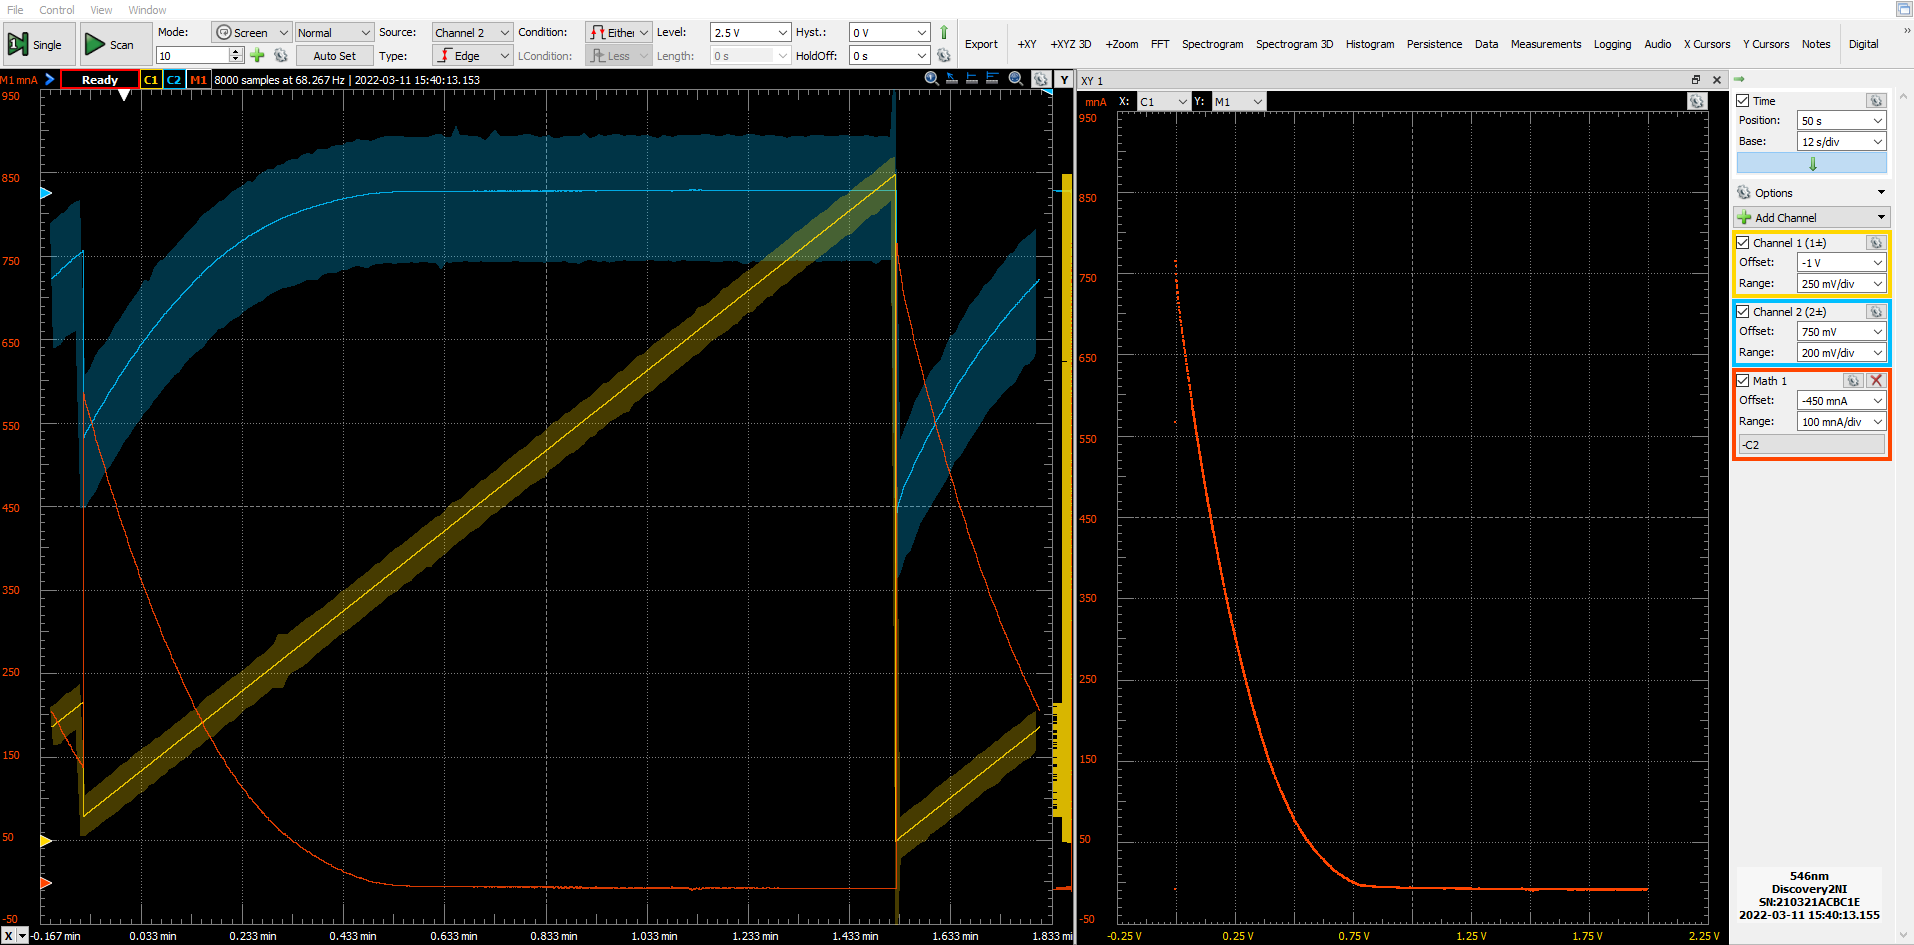
\includegraphics[width=\textwidth]{546nm}
    \caption{Acquisizione della curva tensione $V\ped{bias}(t)$ (CH1)
    corrente (Math1 in mnA = pA) per lunghezza d'onda $546 \; \si{n\m}$, in
    cui si vede un ginocchio verso $I=0$ intorno a
    $V_0 \approx 0.75 \; \si{\V}$
    \label{fig: 546nm}}
\end{figure}

Ipotizziamo che queste correnti siano dovute alla sovrapposizione di vari
effetti di natura diversa:
\begin{enumerate}
        \item emissione di fotoelettroni dall'anodo, dovuta a imperfezioni nel
        sistema di illuminazione del catodo che può investire anche l'anodo
        (schematizzato in \cref{fig: lamp});
        \item estrazione di elettroni dall'anodo per effetto termoionico
        (corrente oscura).
        \item connessione ohmica tra gli elettrodi dovuta al non perfetto
        isolamento delle guaine di rivestimento dei cavi
        $(R \sim 10^{11-12} \; \si{\ohm})$.
    \end{enumerate}

Nonostante ci aspettiamo contributi di gran lunga minoritari rispetto alla
fotocorrente in assenza di bias tra gli elettrodi, già da adesso notiamo come
i primi due crescano con la tensione di frenamento (per questi elettroni il
campo elettrico è accelerante) diventando sempre più significativi,
specialmente per tensioni prossime a quella di azzeramento $V_0$ dove
$I_{ph}$ si estingue.

Per poter ovviare a queste contaminazioni date dalle correnti inverse
$I = I_{ph} + I\ped{inv}$, ne teniamo conto misurandone l'intensità, la quale
supponiamo per semplicità linearmente dipendente dalla tensione di bias
\begin{equation}\label{eq: I0fit}
I\ped{inv} = bV + I_0
\end{equation}

per cui ci aspettiamo che i parametri $b$ e $I_0$ non dipendano dalla
frequenza della luce incidente, ma puramente dalle caratteristiche fisiche
della cella fotoelettrica. Nel caso particolare la corrente inversa fosse di
natura puramente ohmica ci aspettiamo proporzionalità diretta
$I\ped{inv} \propto V\ped{bias}$ e offset $I_0$ nullo.

Assumendo una distribuzione di Fermi-Dirac per gli elettroni liberi nella
banda di conduzione del catodo, senza tenere conto dell'interazione con i
fotoni, possiamo modellare l'andamento della fotocorrente in funzione della
tensione di frenamento come una legge di potenza che si annulla\footnote{
indicando con $\theta(x)$ la funzione gradino di Heaviside $\theta(x) \coloneqq
\begin{cases} 1 & x > 0 \\ 0 & x \leq 0 \end{cases}$} in $V_0$
\[
I_{ph} = (V_0 - V)^{3/2} \theta(V_0 - V)
\]

Dunque possiamo ottenere una misura più attendibile della tensione di
azzeramento -per ogni valore della lunghezza d'onda- tramite fit alla corrente
complessiva, con un modello del tipo:
\begin{equation}\label{eq: Ifit}
I(V) = I_{ph} + I\ped{inv} = a(V_0 - V)^\alpha \theta(V_0 - V) + bV + I_0
\end{equation}

Come prima è ragionevole assumere che l'esponente $\alpha$ sia indipendente
dalle caratteristiche della luce incidente (visto che fisicamente dipende
dalla densità degli stati elettronici del metallo nella banda di conduzione e
da effetti legati all'interazione dei fotoelettroni con il bulbo della
fotocella).

Mentre il parametro $a$, legato alla normalizzazione della fotocorrente,
dovrebbe racchiudere la dipendenza dalla frequenza della luce incidente, poiché
vi dipendono sia l'intensità spettrale della lampada nella banda di selezione
del filtro, che la sezione d'urto dell'effetto fotoelettrico alla
corrispondente energia.

%=======================
\section{Descrizione delle misure}
Nella realizzazione pratica dell'esperimento la radiazione luminosa è
inizialmente emessa secondo uno spettro -praticamente- continuo da una
lampada a LED, viene collimato da un diaframma circolare, dunque focalizzato
da un paio di lenti convergenti prima di essere filtrato e incidere sul catodo
della fotocella (come visto in \cref{fig: lamp}).
\begin{figure}[htbp]
    \centering
	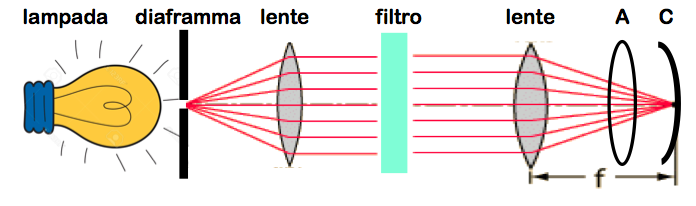
\includegraphics[scale=0.7]{lamp}
    \caption{Rappresentazione schematica dell'apparato di illuminazione della
    fotocella
    \label{fig: lamp}}
\end{figure}

Per variare la frequenza $\nu$ della radiazione che illumina la cella
fotoelettrica utilizziamo 4 filtri di tipo interferenziale, per cui la luce
trasmessa non è monocromatica, ma viene dispersa intorno al valore nominale
centrale secondo una distribuzione di intensità spettrale pressoché uniforme
su intervalli di larghezza $\text{FWHM} \approx 10 \; \si{n\m}$ attorno alla
lunghezza d'onda centrale CWL.

Teniamo conto della dispersione dello spettro incidente associando alla
lunghezza d'onda centrale (riportata nei rispettivi datasheet) un'incertezza
pari alla deviazione standard della curva di trasmissione a partire dalla
larghezza a metà altezza FWHM (anch'essa tabulata) secondo la formula
\[
\lambda \pm \sigma_\lambda = \text{CWL} \pm \text{FWHM}/\sqrt{12}
\]

Per variare la tensione $V\ped{bias} \in [0, 2] \; \si{\V}$, intervallo entro
il quale ci aspettiamo di trovare la tensione di frenamento critica $V_0$,
generiamo in \verb+WG1+ una rampa di tensione compresa tra i due estremi e la
misuriamo con il \verb+CH1+ dell'oscilloscopio di un AD2 secondo lo schema in
\cref{schm: Imeas}.
Con il secondo canale misuriamo contemporaneamente quella generata dal
convertitore corrente-tensione all'uscita del picoamperometro: nel
nostro setup il fattore di conversione vale $\kappa = \SI{1}{n\A/\V}$
($\pm 0.4 \%$ dato dall'incertezza sulla lettura della corrente)
per cui misuriamo $I = \kappa V_{CH2} = V \cdot 10^{-9} \; [\si{A}]$
\begin{figure}[htbp]
    \centering
	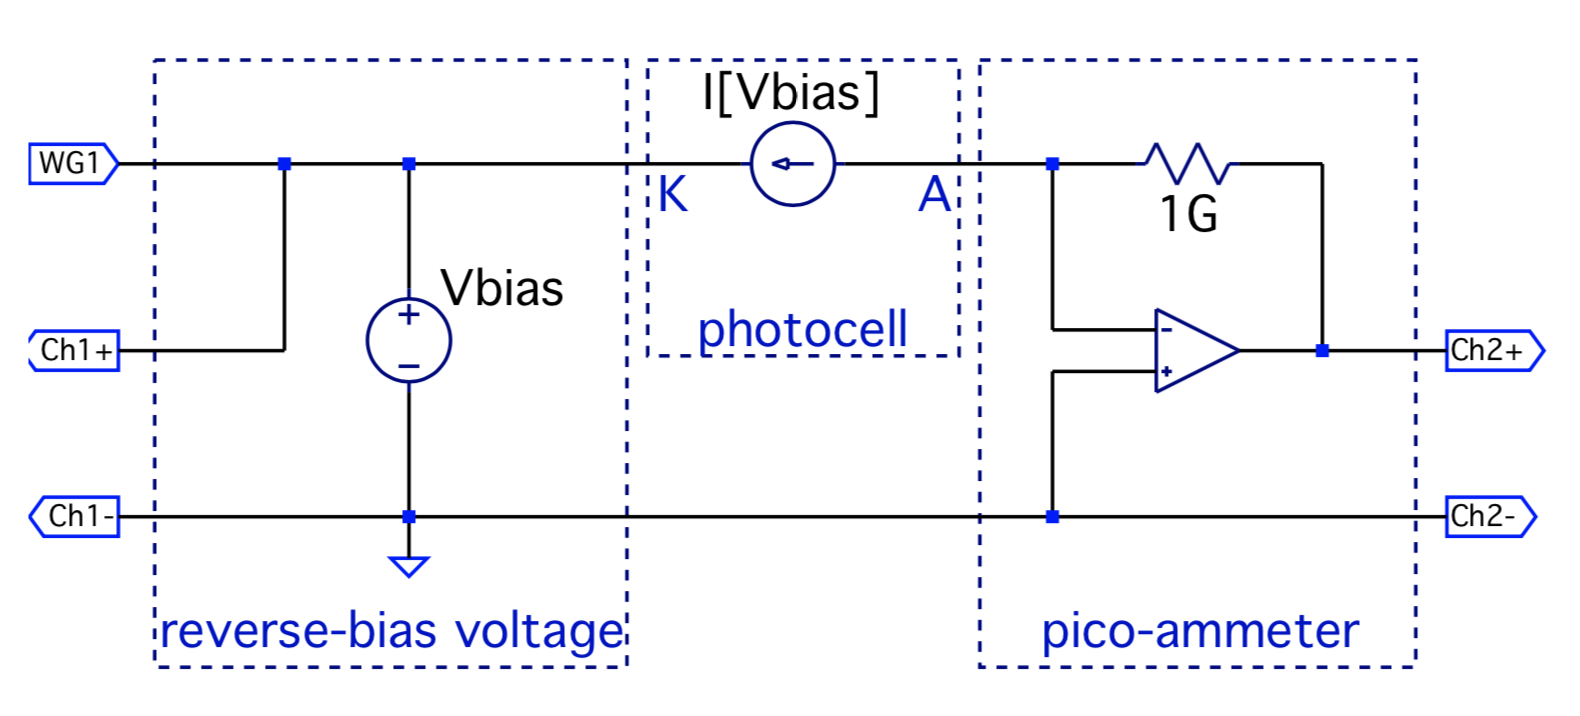
\includegraphics[scale=0.2]{schm}
    \caption{Schema del circuito equivalente per la misura dell'energia
    cinetica dei fotoelettroni.
    \label{schm: Imeas}}
\end{figure}

Finalmente usiamo la funzionalità di plot XY dell'oscilloscopio per ottenere
i grafici della corrente che attraversa la fotocella in funzione della
tensione di bias (come riportato a destra di \cref{fig: 546nm} in rosso le
ordinate Math1, sulle ascisse $V\ped{bias}$ misurata da CH1).

\subsection{Misura della corrente inversa}
Per effettuare la misura della corrente inversa abbiamo acquisito i dati come
sopra con la lampada accesa, con la sola differenza che il vano della
fotocella è stato opportunamente oscurato con un setto opaco, ricavando così
l'andamento della corrente inversa in funzione della tensione di bias nello
stesso intervallo di misura della fotocorrente riportato in \cref{fig: dark}
\begin{figure}[htbp]
    \centering
	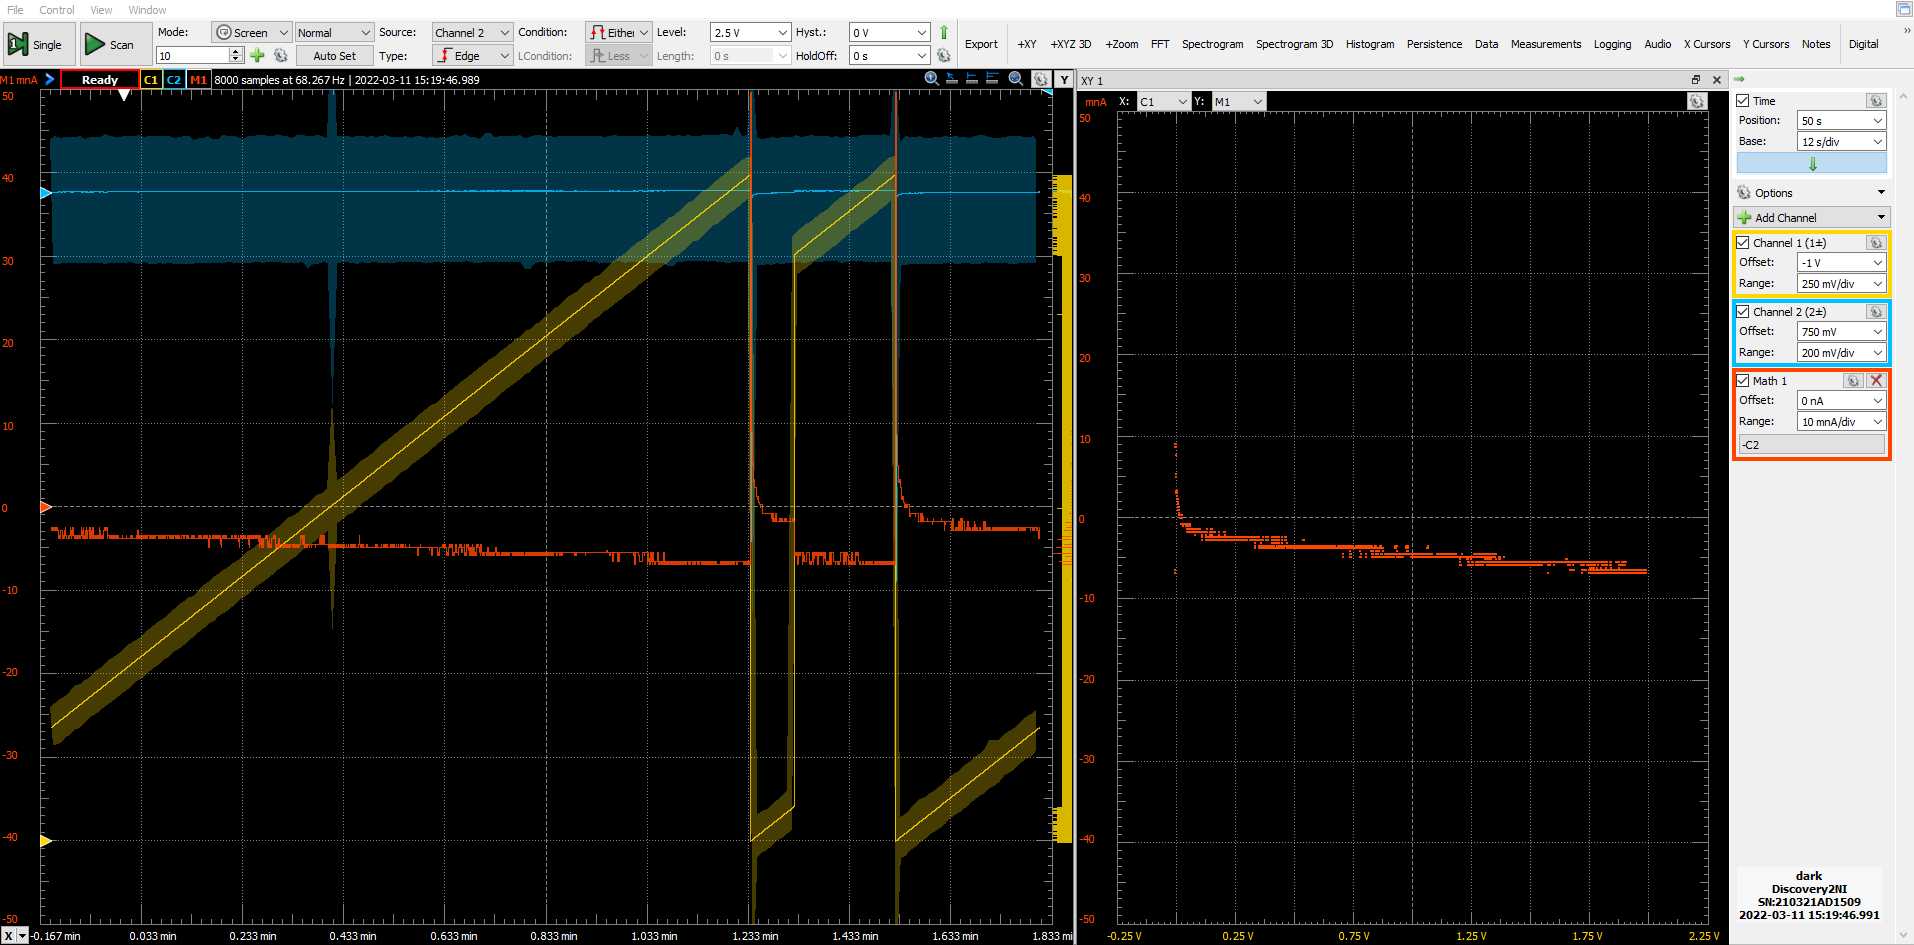
\includegraphics[width=\textwidth]{dark}
    \caption{Stampa a schermo dell'oscilloscopio per la misura della corrente
    senza luce incidente sulla cella fotoelettrica. Una volta superato il
    transiente iniziale all'inizio della rampa di tensione è già possibile
    notare un andamento lineare dei dati.
    \label{fig: dark}}
\end{figure}

%=======================
\section{Analisi dati e stima del rapporto $h/e$}
La stima del rapporto $h/e$ è stata poi ottenuta in due modi diversi: dal coefficiente angolare della retta di \emph{best-fit} da una stima preliminare e dal metodo della corrente inversa.

Assumendo $e = 1.602176634 \times 10^{-19}{\coulomb} $ e $h = \si 6.62607015 \times 10^{-34} \; \si{\J\s} $ il valore atteso del loro rapporto è
\begin{equation}\label{eq: e/h}
\left(\frac{h}{e}\right)\ped{exp} = 4.14 \times 10^{-15} \; \si{\V\s}
\end{equation}

\subsection{Metodo della corrente inversa}
Da un fit lineare alla corrente inversa si ricava
m = -2.58 +- 0.10
q = -1.78 +- 0.13
Chi square/ndof = 92.4/7945
Equivalent resistance 1/m = 388.333157 +- 15.527957 Gohm
corr=-0.8580018344212901

Da un primo fit con \cref{eq: Ifit} lasciando tutti i parametri liberi si
trova
\begin{table}
\centering
\begin{tabular}{ccccccc}
\toprule
$\lambda \; [\si{n\m}]$ & $a \; [\si{p\A/\V^\alpha}] $ & $V_0 \; [\si{m\V}]$ &
$\alpha$ [arb. un.] & $b \; [\si{p\mho}]$ & $I_0 \; [\si{pA}]$ & $\chi^2/\text{ndof}$ \\
\midrule
$450 \pm 3$ & $492 \pm 3$ & $1273 \pm 2$ & $2.264 \pm 0.007$ & $-4.4 \pm 0.5$ &
$-0.6 \pm 0.8$ & $599/7817$ \\
$499 \pm 3$ & $756 \pm 4$ & $1061 \pm 2$ & $2.441 \pm 0.009$ & $-3.1 \pm 0.4$ &
$-2.5 \pm 0.6$ & $555/7817$ \\
$546 \pm 3$ & $1066 \pm 6$ & $863 \pm 3$ & $2.547 \pm 0.012$ & $-2.6 \pm 0.3$ &
$-2.9 \pm 0.4$ & $368/7817$ \\
$577 \pm 3$ & $1595 \pm 8$ & $751 \pm 3$ & $2.603 \pm 0.016$ & $-2.4 \pm 0.2$ &
$-3.2 \pm 0.3$ & $210/7817$ \\
\bottomrule
\end{tabular}
\end{table}

\subsection{Stima dell'esponente $\alpha$}
Si è notato che la stima dei valori del potenziale frenante critico e
dell'esponente $\alpha$ esibivano una apprezzabile dipendenza dall'intervallo
di tensioni di bias considerate nel fit della fotocorrente.

Considerando valori di $V_{bias} \sim 0$, oltre
a quelle vicine al ginocchio in $V_{0}$, si è visto che il valore
dell'esponente $\alpha$ assume un andamento monotono crescente in funzione
della lunghezza d'onda in maniera analoga a quanto osservato finora per il
parametro $a$.

Si è scelto quindi di fissare il valore di $\alpha$ come media pesata dei
valori ottimali stimati dai fit prendendo in considerazione l'intero range di
tensioni esplorato, dunque di eseguire un nuovo fit ai 4 dataset lasciando
liberi solamente i restanti parametri dipendenti dalla frequenza della luce
incidente: $V_{0}$ e $a$.

In particolare, dal fit con alpha libero si trova
np.mean(alphas)
Out[27]: 2.4806408028824034

np.mean(dalphas)
Out[28]: 0.010212701821352213

1/pars[0]
Out[29]: 3.568317911720477
Quindi un valore del rapporto h/e sottostimato di circa il $15 \%$ rispetto al
valore atteso.

Mentre dai valori di $V_{0}$ ricavati fissando $\alpha$ proponiamo un fit
lineare alla relazione inversa
\begin{equation}
\nu = \frac{e}{h} V_{0} - W_{0}/h
\end{equation}
da cui otteniamo come valore del rapporto $h/e = 4.19 \pm 0.13 \; \si{\V \s}$,
che è compatibile entro l'incertezza con il valore tabulato di 4.14.

%=======================
\section{Valutazione degli effetti sistematici}
In realtà il nostro apparato è racchiuso da una scatola metallica per
schermarlo dalla luce e dal rumore elettronico ambientale, ma la misura
di $h/e$ è affetta da diverse fonti di errore sistematico.

\subsection{Effetto fotoelettrico sull'anodo}
Dal datasheet della cella fotoelettrica sappiamo che questa è composta da un
anodo in lega di platino e rodio, che è una spira di $SI{3}{c\meter}$ e da un
catodo in potassio rivestito di ossido d'argento, costituito da un arco
delle dimensioni di $\SI{4}{c\meter}$.

Per minimizzare il contributo alla corrente inversa dato dall'emissione di
fotoelettroni dall'anodo quando viene investito dagli aloni del fascio di
luce incidente si è ridotta l'apertura del diaframma così che la sua
immagine, messa a fuoco al centro del catodo, abbia dimensioni molto
inferiori al raggio dell'anodo.

Non solo: il potassio -come tipico per i metalli alcalini- ha lavoro di
estrazione $W\ped{0, K} \approx 2.15 \; \si{\V}$ più basso di quello di altri
metalli, come il platino $W\ped{0, Pt} \approx 5.29 \; \si{\V}$ con cui è
stato realizzato l'anodo sempre per questo motivo.

\subsection{Effetto termoionico e connessione ohmica tra gli elettrodi}
A differenza del caso precedente ci sono due effetti che non possono
essere soppressi altrettanto facilmente, per cui ci aspettiamo forniscano
il contributo maggioritario alla corrente inversa:
\begin{itemize}
    \item L'effetto termoionico si ha sia sul catodo che sull'anodo e diventa pià significativo all'aumentare della tensione di \emph{bias}. La corrente $ I\ped{inv} $ misurata per $ V > V\ped{0}$ è principalmente attribuibile a questo contributo e dovrebbe essere osservabile (e quindi quantificabile in modo più preciso) anche in assenza di illuminazione;

    \item I cavi coassiali uscenti dalla scatola metallica in cui è contenuto l'apparato sono connessi al catodo e all'anodo e poi esternamente collegati rispettivamente in parallelo al voltmetro e in serie al picoamperometro. La scatola metallica scherma dal rumore elettronico, ma le guaine di rivestimento dei cavi non sono perfettamente isolanti e questo può comportare una ulteriore corrente inversa tra gli elettrodi, che per via dell'ordine di grandezza delle correnti in gioco, diventa non trascurabile.
\end{itemize}

\subsection{Considerazioni sul metodo \texttt{A}}
Nel \hyperref[sec:metodoA]{metodo \texttt{A}} si determina il valore della corrente inversa interpolando le misure nella regione $I \leq 0 $ con un modello lineare. I parametri $ b $ e $ I_{0} $ non dovrebbero dipendere dalla lunghezza d'onda della radiazione incidente: considerando un modello del tipo equazione di Shockley per un diodo a giunzione per la fotocellula, il modello lineare dovrebbe essere uno sviluppo al primo ordine dell'equazione caratteristica nel range considerato, con $ b $ parametro nell'esponenziale e $ I_{0} $ valore asintotico della corrente.

Tuttavia dalla~\eqref{fig:fit-oscuro} è possibile notare come $ I\ped{inv} $ abbia in realtà andamenti diversi al variare della lunghezza d'onda: per le lunghezze d'onda minori, quindi per fotoni più energetici, il potenziale di frenamento $ V_{0} $ è più elevato e dunque la corrente tende più lentamente al valore asintotico. Questo comporta una deviazione significativa dall'andamento lineare e dunque i parametri del \emph{fit} manifestano necessariamente una dipendenza dalla lunghezza d'onda impiegata.

\subsection{Considerazioni sul metodo \texttt{B}}
Nel \hyperref[sec:metodoB]{metodo \texttt{B}} si adopera l'equazione~\eqref{eq:modello-magico} e in tale caso i parametri $ b $ e $ I_{0} $ risultano compatibili. Nella zona di transizione $ V\sim V_{0} $, il parametro $ a $ tiene conto della dipendenza dalla lunghezza d'onda: dai parametri di \emph{best-fit} si nota infatti che $ a $ cambia significativamente al variare della lunghezza d'onda ed è monotona crescente nella lunghezza d'onda.

L'origine fisica del parametro $\alpha$ nella legge di potenza può essere compresa descrivendo, in prima approssimazione, il gas di elettroni nella banda di conduzione del metallo alcalino di cui è costituito il catodo come un gas degenere di Fermi: ovviamente questo modello considera gli elettroni nel metallo come liberi e non tiene conto delle successive interazioni dei fotoelettroni con il bulbo della fotocella. Si ottengono infatti valori maggiori di $ 3/2 $, gli $ \alpha $ di \emph{best-fit} non risultano compatibili tra loro e risultano monotoni crescenti nella lunghezza d'onda.



%=======================
\section*{Conclusioni e commenti finali}
Si è riusciti a dare una misura ragionevole del rapporto carica/massa
dell'elettrone a partire da un'analisi delle fotografie della sua traiettoria
elicoidale in presenza di un campo magnetico uniforme.

%=======================
\section*{Dichiarazione}
I firmatari di questa relazione dichiarano che il contenuto della relazione \`e
originale, con misure effettuate dai membri del gruppo, e che tutti i firmatari
hanno contribuito alla elaborazione della relazione stessa.

%=======================
\begin{thebibliography}{1}
\bibitem{Coope}{I. D. Coope, Circle fitting by linear and nonlinear least
squares, Department of Mathematics, University of Canterbury, Christchurch,
New Zealand, N.60, May, 1992,
\url{https://ir.canterbury.ac.nz/bitstream/handle/10092/11104/coope_report_no69_1992.pdf?sequence=1&isAllowed=y}}
\end{thebibliography}

\end{document}
